\documentclass[a4paper, 11pt]{article}
\usepackage{geometry}
\usepackage{url}
\usepackage{booktabs}
\usepackage{color}
\usepackage{graphicx}
\linespread{1}

\geometry{a4paper,top=3cm,left=3cm,right=2.5cm,bottom=2cm}

\usepackage{hyperref}
\hypersetup{colorlinks,linkcolor=black,citecolor=blue}

\title{\textbf{Laboratory assignment} \\[1ex] \large \textbf{Component} {2}}

\author{\textbf{Authors:} {Ichim Stefan, Mirt Leonard}\\ \textbf{Group:} {246/1}}

\begin{document}

\maketitle

\section{Data Analysis}
First, to be able to take statistics from features, we made sure that all the features are in numeric form. We tranformed the ocean proximity feature into a numeric features as follows:
'$<$ 1H OCEAN': 0, 
'INLAND': 1, 
'ISLAND': 2, 
'NEAR BAY': 3, 
'NEAR OCEAN': 4.

\begin{table}[h!]
\centering
\caption{Statistical Summary of Features}
\begin{tabular}{lrrrrrr}
\toprule
\textbf{Feature} & \textbf{Count} & \textbf{Mean} & \textbf{Std} & \textbf{Min} & \textbf{Max} \\
\midrule
Longitude         & 20640 & -119.57 & 2.00 & -124.35 & -114.31 \\
Latitude          & 20640 & 35.63   & 2.14 & 32.54   & 41.95   \\
Housing Age       & 20640 & 28.64   & 12.59 & 1.00   & 52.00   \\
Total Rooms       & 20640 & 2635.76 & 2181.62 & 2.00 & 39320.00 \\
Total Bedrooms    & 20433 & 537.87  & 421.39 & 1.00   & 6445.00 \\
Population        & 20640 & 1425.48 & 1132.46 & 3.00  & 35682.00 \\
Households        & 20640 & 499.54  & 382.33 & 1.00   & 6082.00 \\
Median Income     & 20640 & 3.87    & 1.90 & 0.50    & 15.00   \\
Median House Value & 20640 & 206855.82 & 115395.62 & 14999.00 & 500001.00 \\
Ocean Proximity   & 20640 & 1.17    & 1.42 & 0.00    & 4.00    \\
\bottomrule
\end{tabular}
\end{table}

\subsection{Pearson Test: Data Correlation and Independence}
% \begin{figure}[h]
%     \centering
%     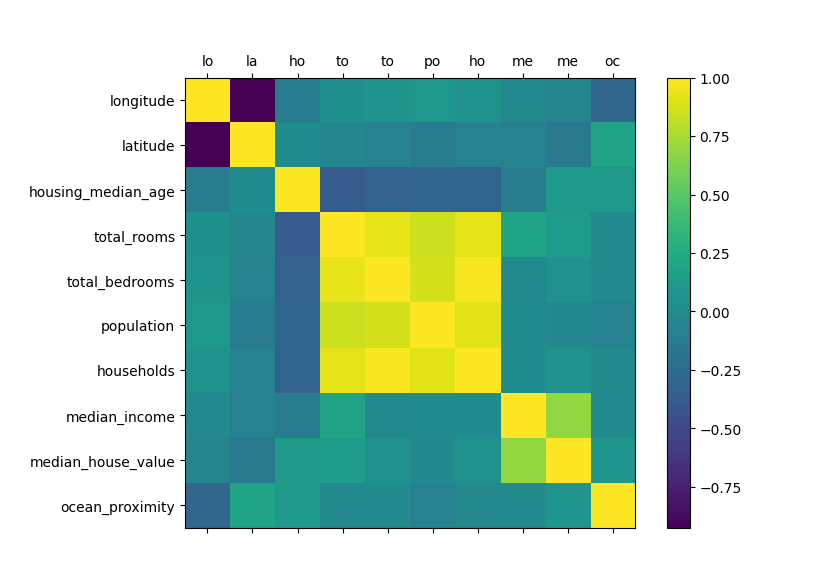
\includegraphics[width=1\linewidth]{figs/correlation.png}
%     \caption{Pearson test results: 1 - strong positive, -1 - strong negative, 0 - no connection}
%     \label{fig:correlation}
% \end{figure}
\begin{figure}[h]
    \centering
    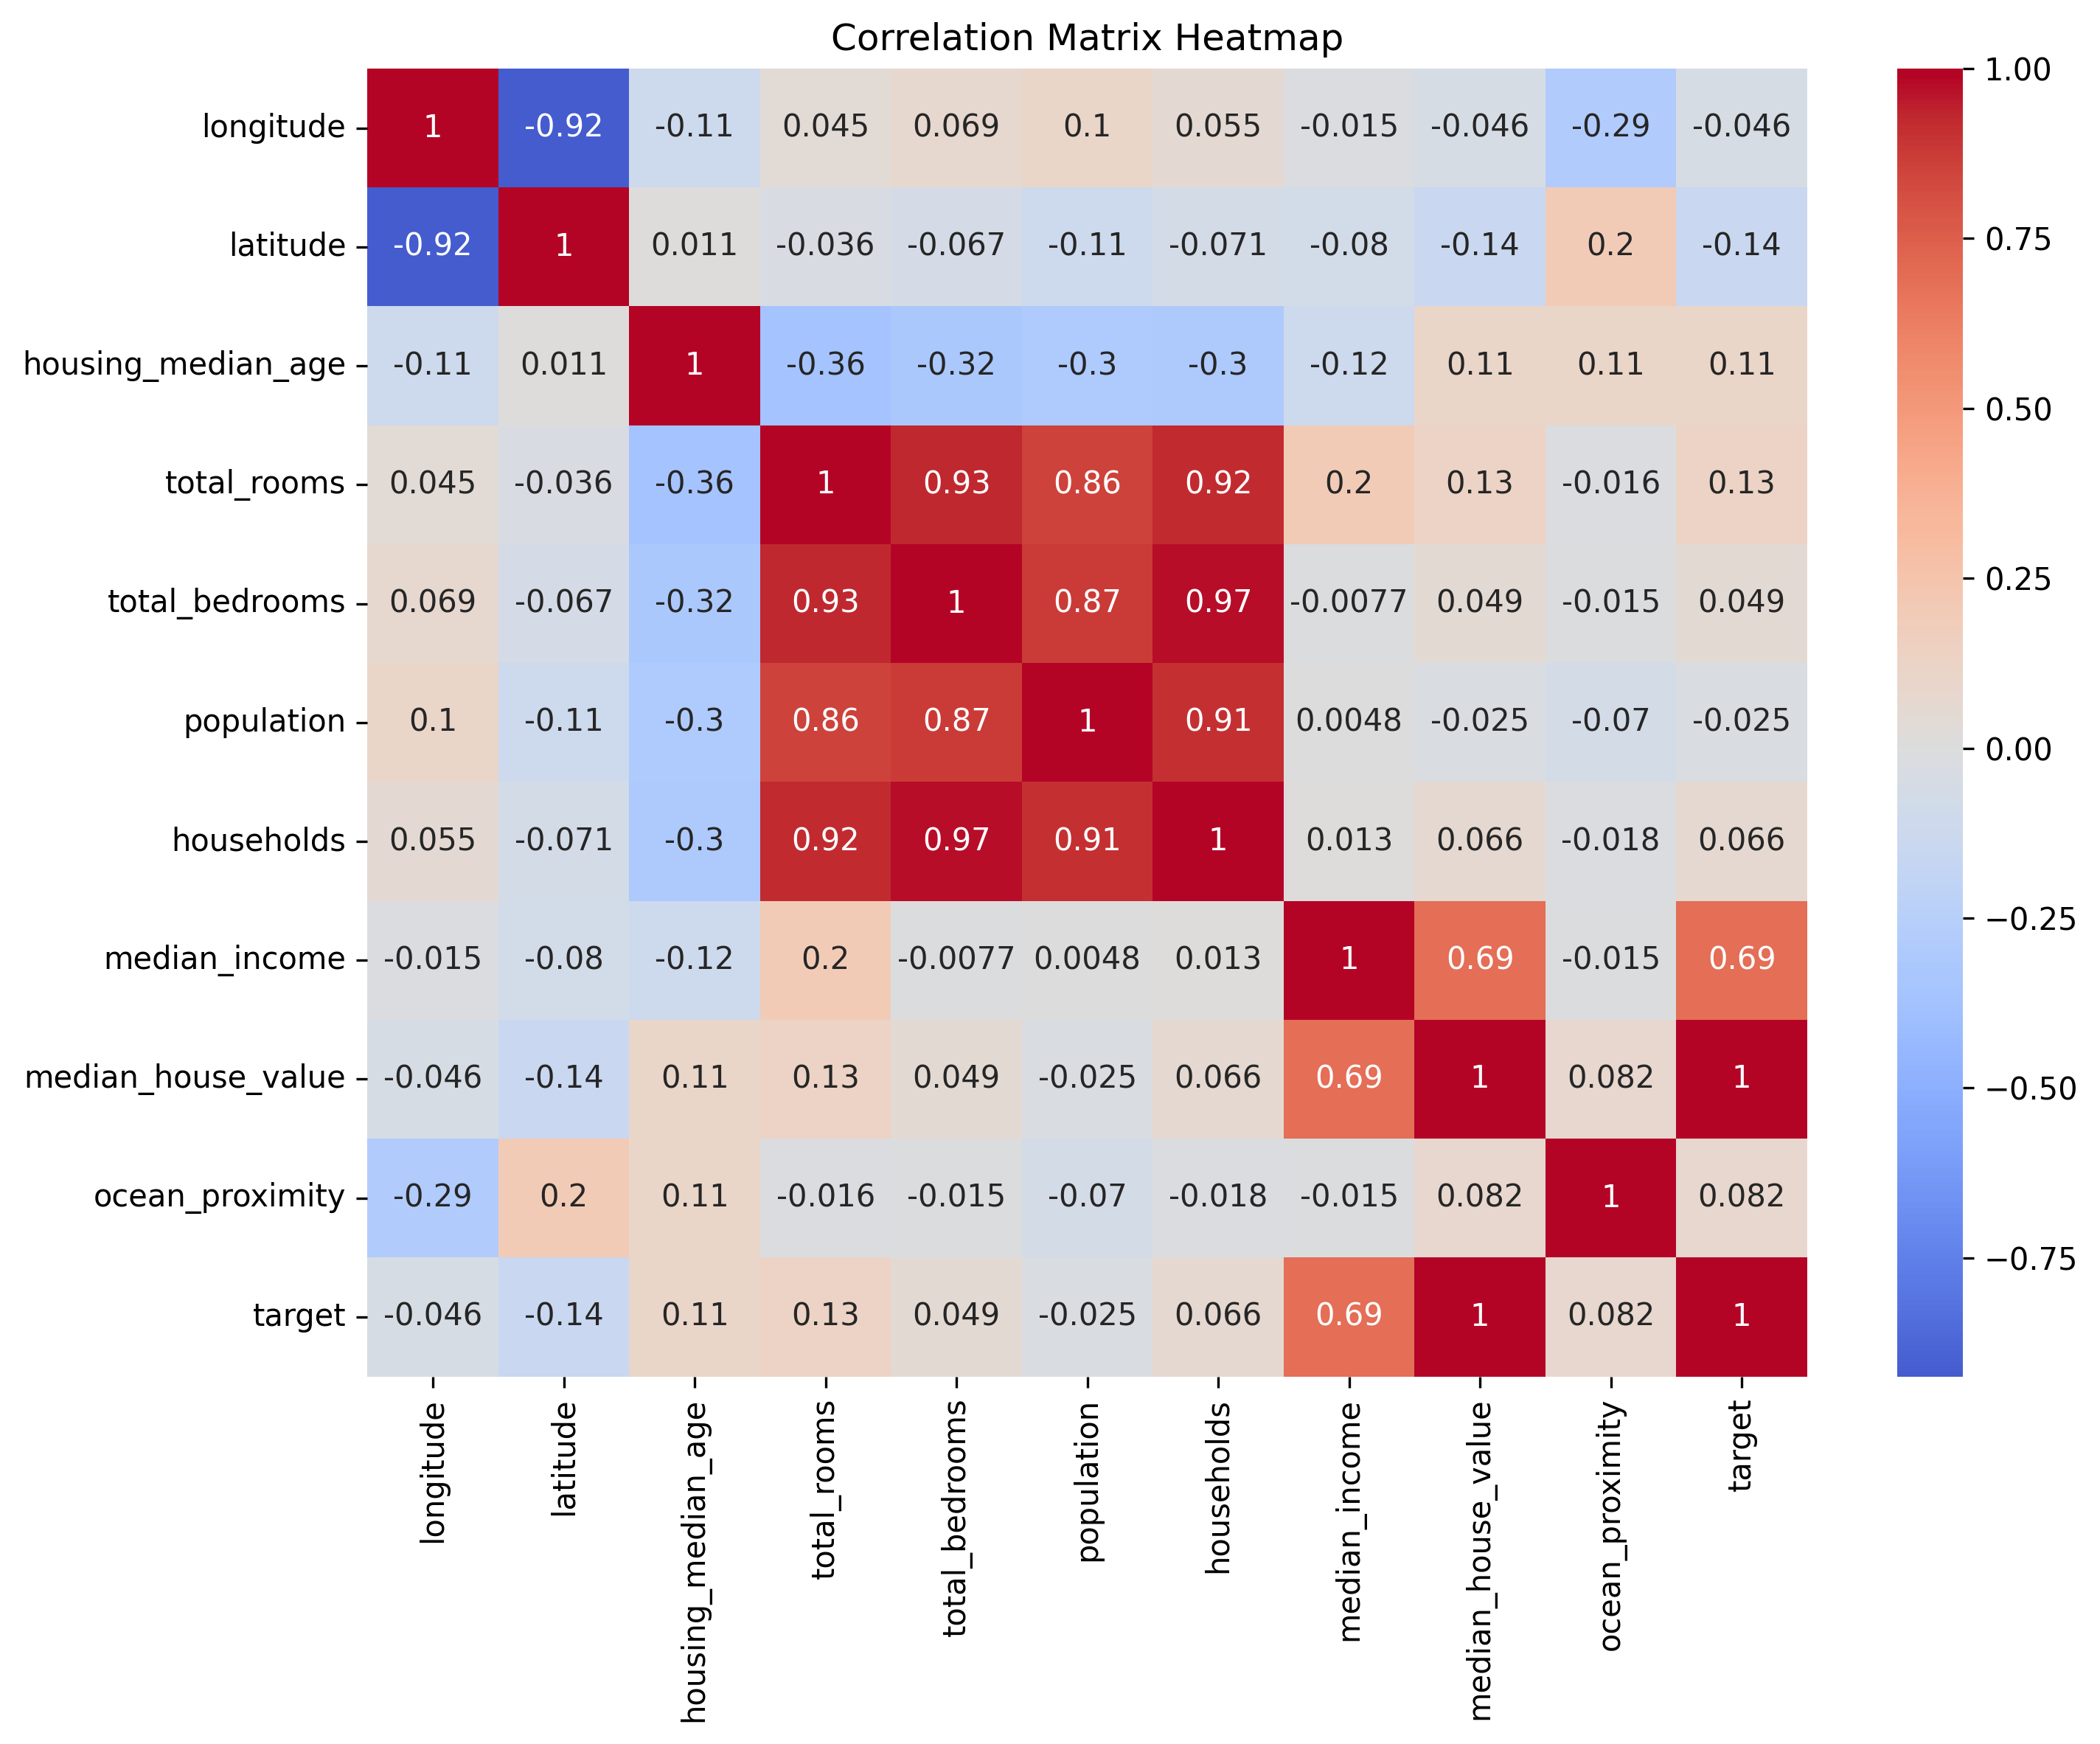
\includegraphics[scale=0.5]{figs/correlation_heatmap.png}
    \caption{Pearson test results: 1 - strong positive, -1 - strong negative, 0 - no connection}
    \label{fig:correlation_heatmap}
\end{figure}

The correlation heatmap reveals several important relationships in our dataset. Most notably, median income shows the strongest positive correlation with house values (0.688), indicating that areas with higher incomes tend to have higher house prices. There are also moderate correlations between related features such as total rooms and total bedrooms, and households and population, which is expected. Interestingly, geographic features (longitude and latitude) show relatively weak correlations with house values, suggesting that location alone is not a strong predictor of price.

\subsection{Statistical Tests: Feature Importance}

\begin{table}[h!]
    \centering
    \caption{Statistical Tests for Feature Importance}
    \begin{tabular}{lrrrr}
        \toprule
        \textbf{Feature} & \textbf{Pearson} & \textbf{Spearman} & \textbf{F-Score} & \textbf{Mutual Information} \\
        \midrule
        Median Income & 0.688 & 0.677 & 1.000 & 0.051 \\
        Latitude & 0.144 & 0.166 & 0.024 & 0.049 \\
        Total Rooms & 0.134 & 0.206 & 0.020 & 0.006 \\
        Housing Median Age & 0.106 & 0.075 & 0.013 & 0.004 \\
        Ocean Proximity & 0.082 & 0.133 & 0.007 & 0.028 \\
        Households & 0.066 & 0.113 & 0.005 & 0.004 \\
        Total Bedrooms & 0.049 & 0.086 & 0.003 & 0.003 \\
        Longitude & 0.046 & 0.070 & 0.002 & 0.053 \\
        Population & 0.025 & 0.004 & 0.001 & 0.003 \\
        \bottomrule
    \end{tabular}
\end{table}

We employed multiple statistical tests to evaluate feature importance from different perspectives. The Pearson correlation measures linear relationships, while Spearman captures monotonic relationships that might not be linear. F-Score helps identify discriminative features, and Mutual Information captures both linear and non-linear relationships. Consistently across all metrics, median income emerges as the most significant feature, while population shows the weakest relationship with house values. The variation in rankings across different tests suggests some non-linear relationships in our data.

\subsection{Data Visualization and Interpretation}

\begin{figure}[h]
    \centering
    \begin{minipage}{0.48\textwidth}
        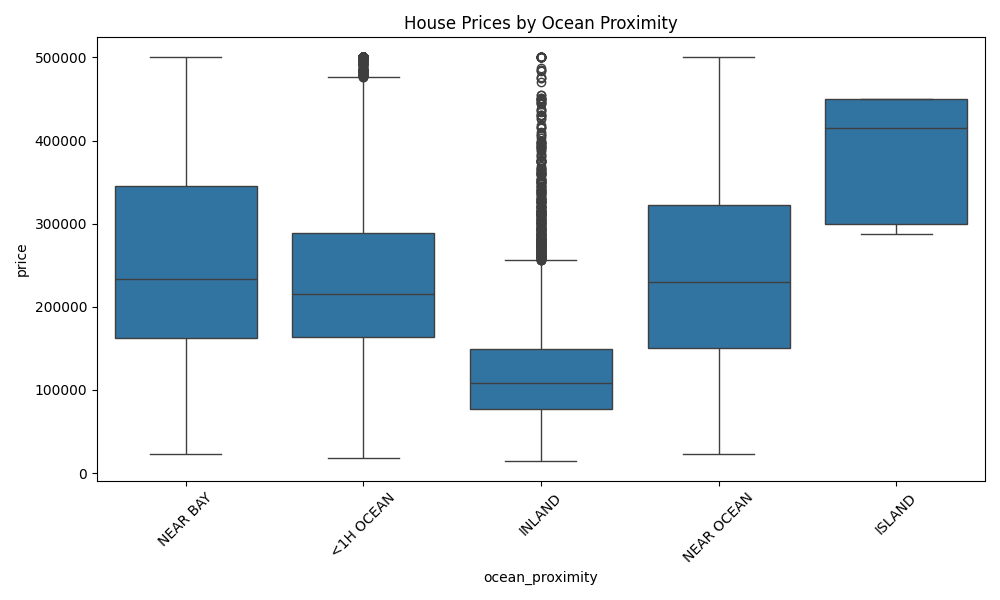
\includegraphics[width=\linewidth]{figs/price_by_ocean.png}
        \caption{House prices variation by ocean proximity}
        \label{fig:price_ocean}
    \end{minipage}
    \hfill
    \begin{minipage}{0.48\textwidth}
        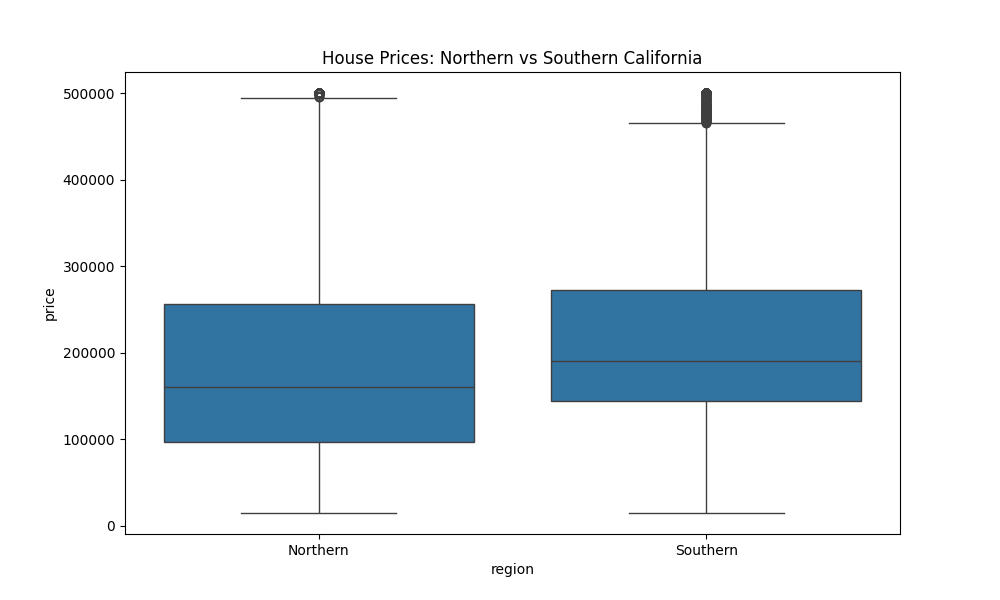
\includegraphics[width=\linewidth]{figs/price_by_region.png}
        \caption{Price comparison: Northern vs Southern California}
        \label{fig:price_region}
    \end{minipage}
\end{figure}

These visualizations reveal significant geographic price variations in the California housing market. Ocean proximity appears to have a substantial impact on house prices, with properties closer to the ocean generally commanding higher values. The north-south comparison demonstrates regional market differences, likely influenced by factors such as local economic conditions and population density.

\begin{figure}[h]
    \centering
    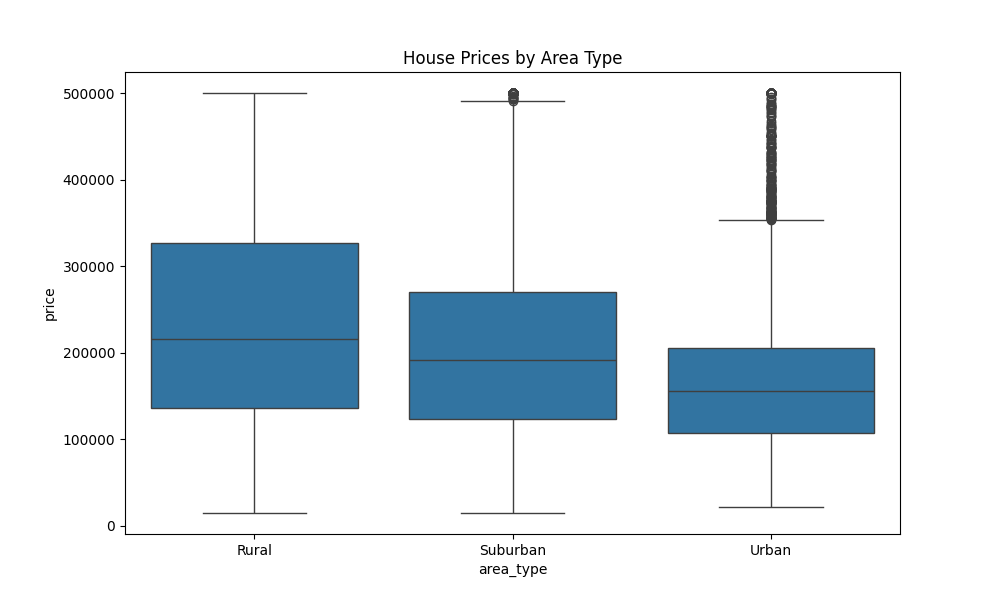
\includegraphics[scale=0.5]{figs/price_by_area_type.png}
    \caption{House prices across different area types}
    \label{fig:price_area}
\end{figure}

The analysis of house prices across different area types reveals distinct pricing patterns based on neighborhood characteristics. This segmentation helps understand how property values vary with urbanization levels and local development patterns.

\begin{figure}[h]
    \centering
    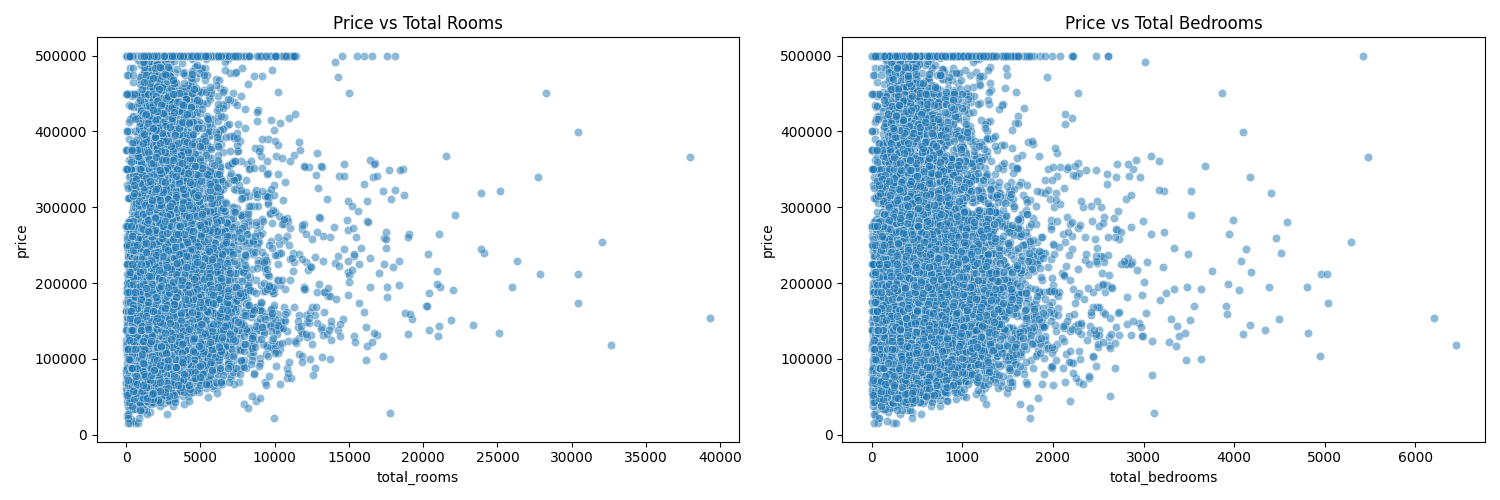
\includegraphics[width=\linewidth]{figs/price_vs_size.png}
    \caption{Relationship between house size and price}
    \label{fig:price_size}
\end{figure}

\begin{figure}[h]
    \centering
    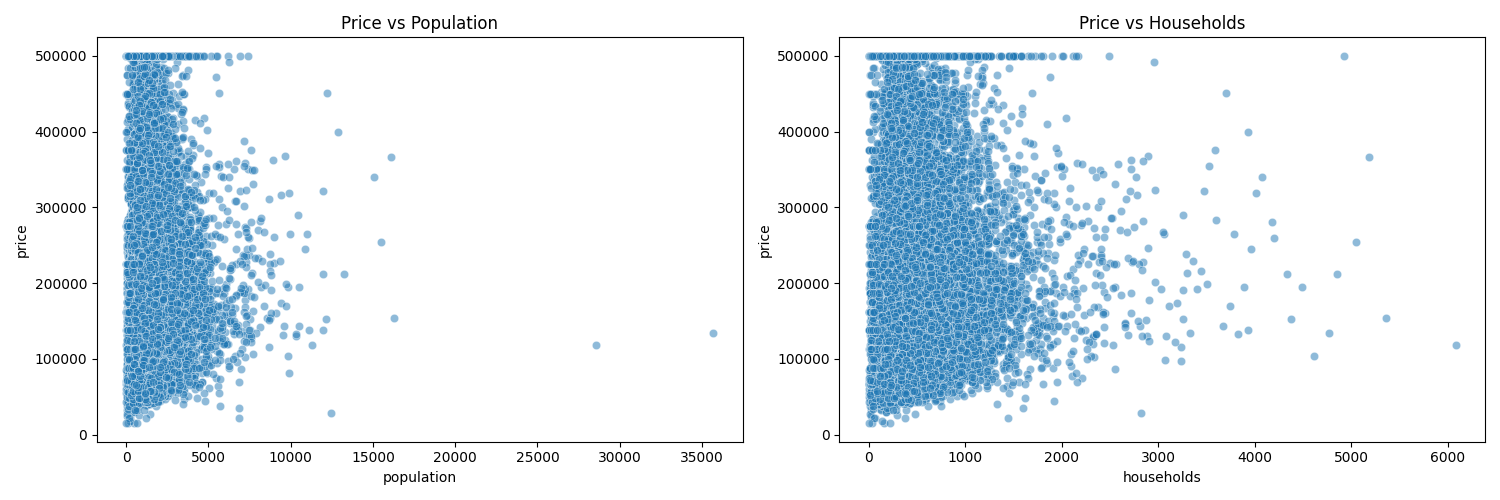
\includegraphics[width=\linewidth]{figs/price_vs_neighborhood.png}
    \caption{Impact of neighborhood characteristics on price}
    \label{fig:price_neighborhood}
\end{figure}

The relationship between house size and price shows a generally positive correlation, though with notable variance. The neighborhood characteristics analysis demonstrates how community features influence property values, highlighting the importance of considering both physical and social factors in price determination.

\begin{figure}[h]
    \centering
    \begin{minipage}{0.48\textwidth}
        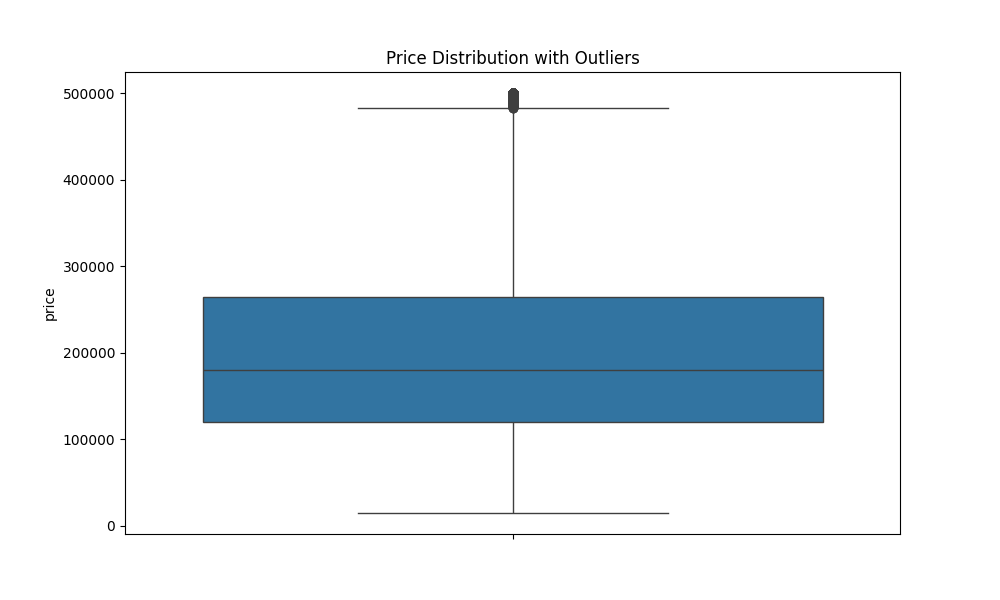
\includegraphics[width=\linewidth]{figs/price_outliers.png}
        \caption{Distribution of price outliers}
        \label{fig:outliers_box}
    \end{minipage}
    \hfill
    \begin{minipage}{0.48\textwidth}
        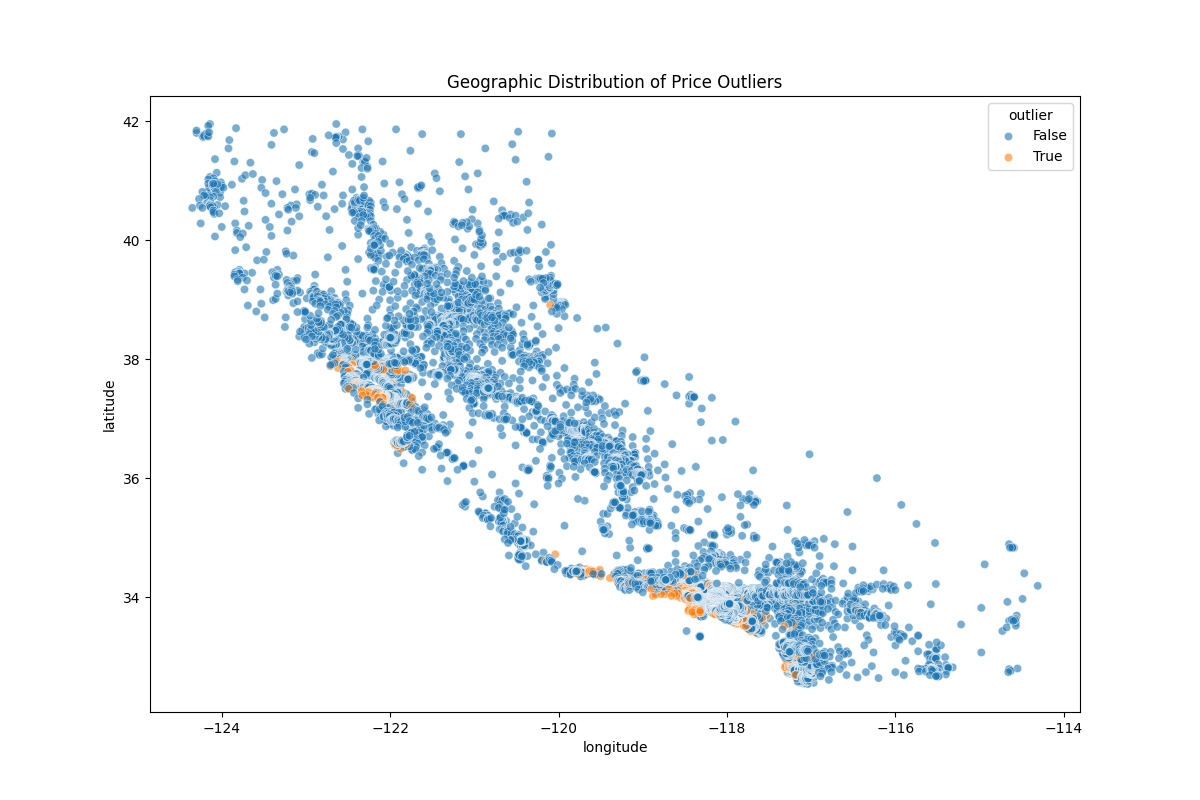
\includegraphics[width=\linewidth]{figs/outliers_geographic.png}
        \caption{Geographic distribution of outliers}
        \label{fig:outliers_map}
    \end{minipage}
\end{figure}

The analysis of price outliers reveals interesting patterns in the California housing market. The box plot distribution helps identify extreme values, while the geographic distribution of these outliers shows they're not randomly distributed but tend to cluster in specific regions, particularly in coastal and metropolitan areas. This suggests that these extreme prices are often driven by location-specific factors rather than just property characteristics.

\begin{figure}[h]
    \centering
    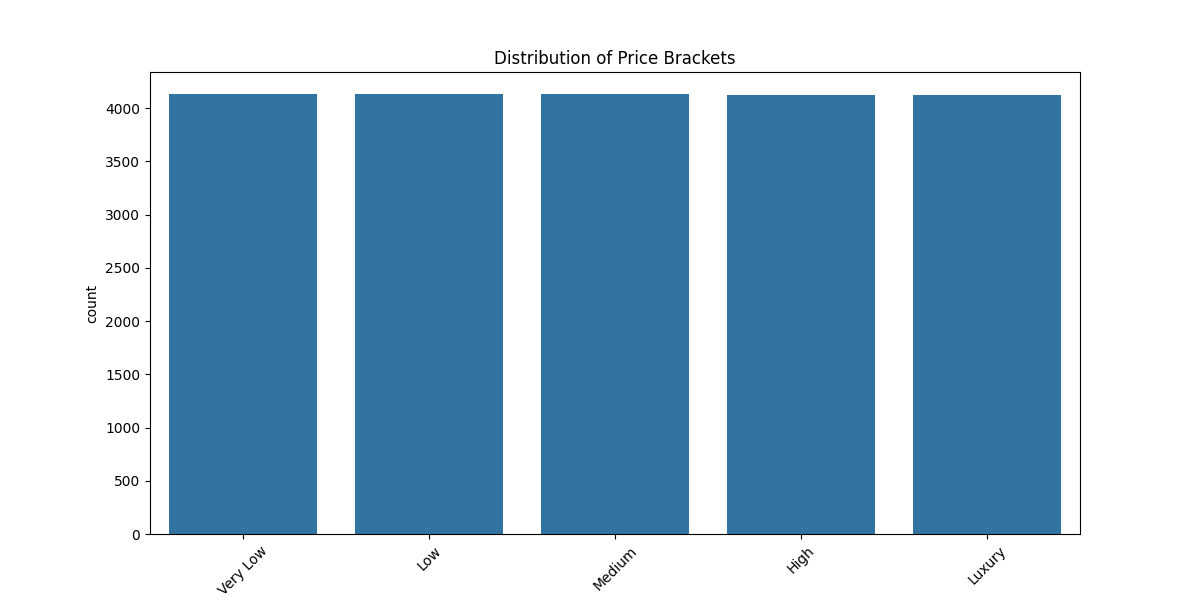
\includegraphics[width=0.8\linewidth]{figs/price_brackets.png}
    \caption{Distribution of properties across price brackets}
    \label{fig:price_brackets}
\end{figure}

\begin{figure}[h]
    \centering
    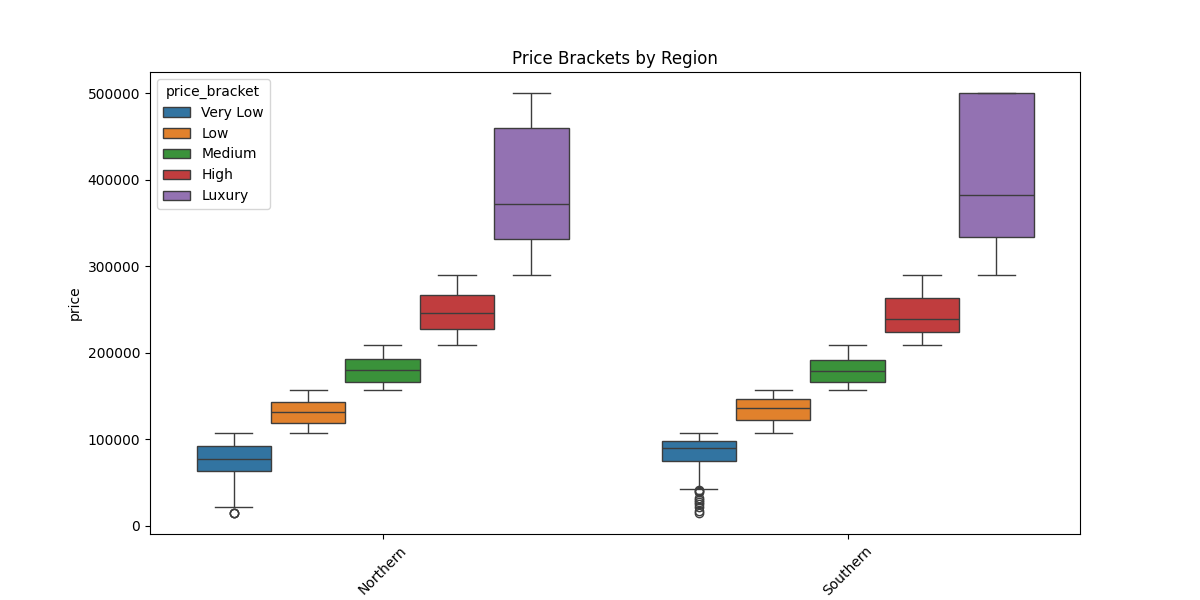
\includegraphics[width=\linewidth]{figs/regional_markets.png}
    \caption{Regional market characteristics by price bracket}
    \label{fig:regional_markets}
\end{figure}

The distribution across price brackets shows the overall market segmentation, with distinct patterns in different price ranges. The regional market analysis further breaks this down by geographic areas, revealing how different regions of California have distinct price distributions and market characteristics. This information is particularly valuable for understanding market accessibility and investment opportunities across different areas.

\subsection{Feature distribution}

\begin{figure}[htbp]
    \centering
    \begin{minipage}{0.45\textwidth}
        \centering
        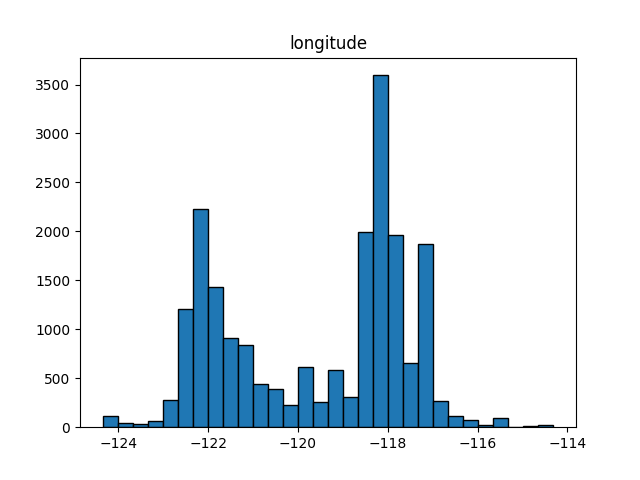
\includegraphics[width=\linewidth]{figs/longitude_distribution.png}
        \caption{Longitude distribution}
        \label{fig:longitude_distribution}
    \end{minipage}\hfill
    \begin{minipage}{0.45\textwidth}
        \centering
        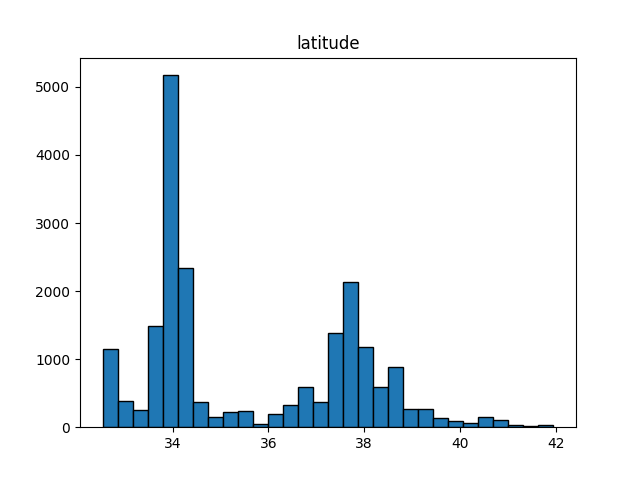
\includegraphics[width=\linewidth]{figs/latitude_distribution.png}
        \caption{Latitude distribution}
        \label{fig:latitude_distribution}
    \end{minipage}
    
    \vspace{0.1cm}  % Adds vertical space between rows
    
    \begin{minipage}{0.45\textwidth}
        \centering
        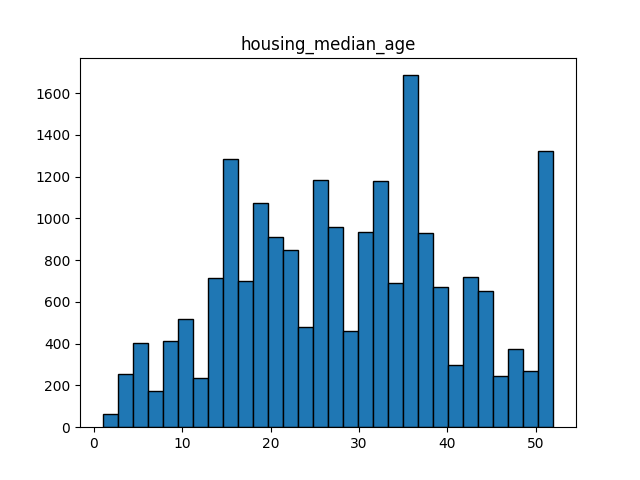
\includegraphics[width=\linewidth]{figs/housing_median_age_distribution.png}
        \caption{Housing median age distribution}
        \label{fig:housing_age_distribution}
    \end{minipage}\hfill
    \begin{minipage}{0.45\textwidth}
        \centering
        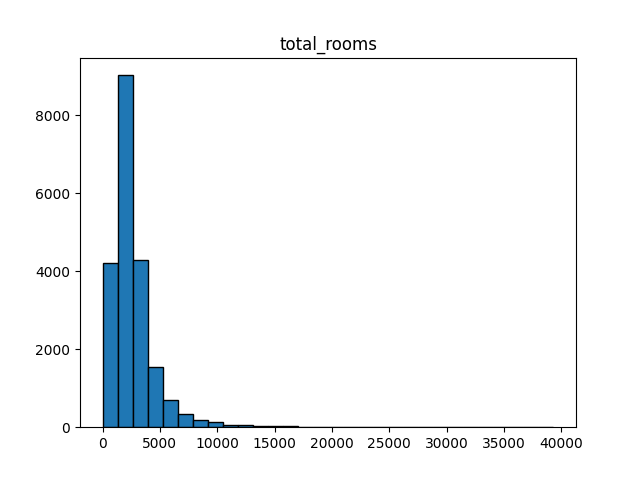
\includegraphics[width=\linewidth]{figs/total_rooms_distribution.png}
        \caption{Total rooms distribution}
        \label{fig:total_rooms_distribution}
    \end{minipage}
    
    \vspace{0.1cm}  % Adds vertical space between rows
    
    \begin{minipage}{0.45\textwidth}
        \centering
        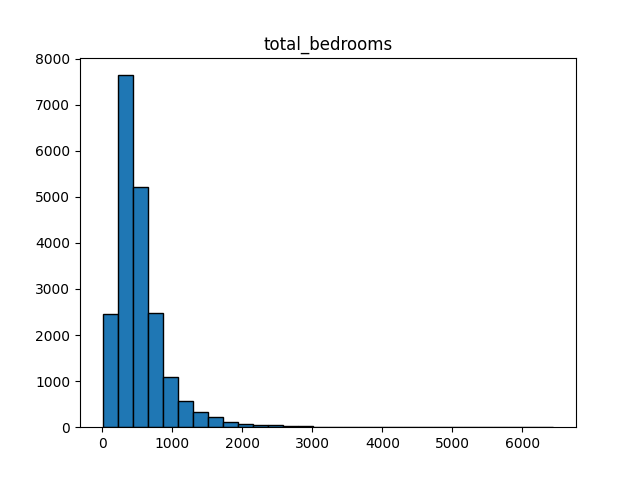
\includegraphics[width=\linewidth]{figs/total_bedrooms_distribution.png}
        \caption{Total bedrooms distribution}
        \label{fig:total_bedrooms_distribution}
    \end{minipage}\hfill
    \begin{minipage}{0.45\textwidth}
        \centering
        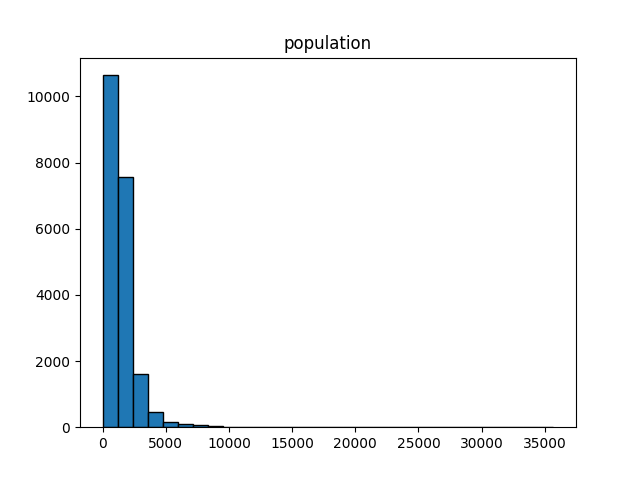
\includegraphics[width=\linewidth]{figs/population_distribution.png}
        \caption{Population distribution}
        \label{fig:population_distribution}
    \end{minipage}
\end{figure}
\begin{figure}[htbp]
    \centering
    \vspace{0.1cm}  % Adds vertical space between rows
    
    \begin{minipage}{0.45\textwidth}
        \centering
        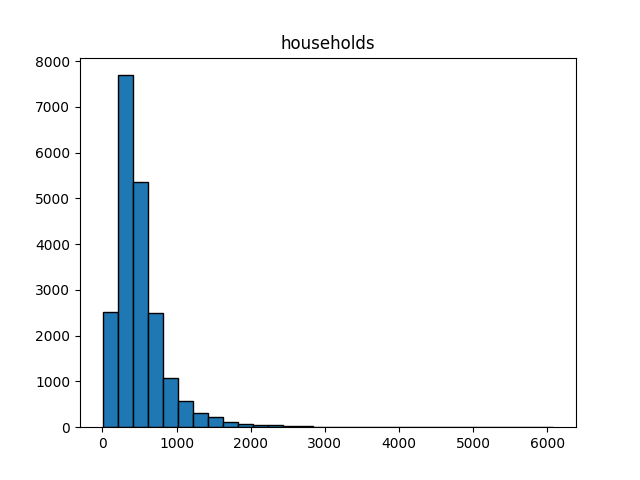
\includegraphics[width=\linewidth]{figs/households_distribution.png}
        \caption{Households distribution}
        \label{fig:households_distribution}
    \end{minipage}\hfill
    \begin{minipage}{0.45\textwidth}
        \centering
        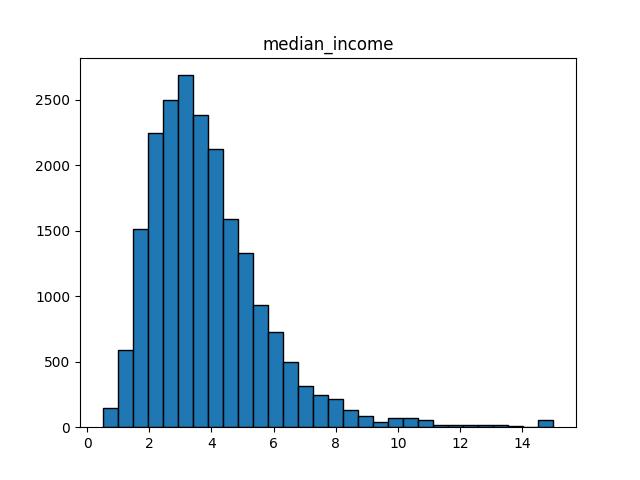
\includegraphics[width=\linewidth]{figs/median_income_distribution.png}
        \caption{Median income distribution}
        \label{fig:median_income_distribution}
    \end{minipage}
    
    \vspace{0.1cm}  % Adds vertical space between rows
    
    \begin{minipage}{0.45\textwidth}
        \centering
        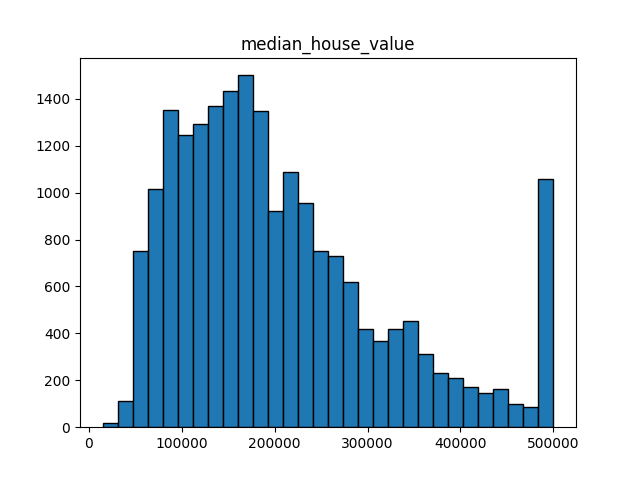
\includegraphics[width=\linewidth]{figs/median_house_value_distribution.png}
        \caption{Median house value distribution}
        \label{fig:median_house_value_distribution}
    \end{minipage}\hfill
    \begin{minipage}{0.45\textwidth}
        \centering
        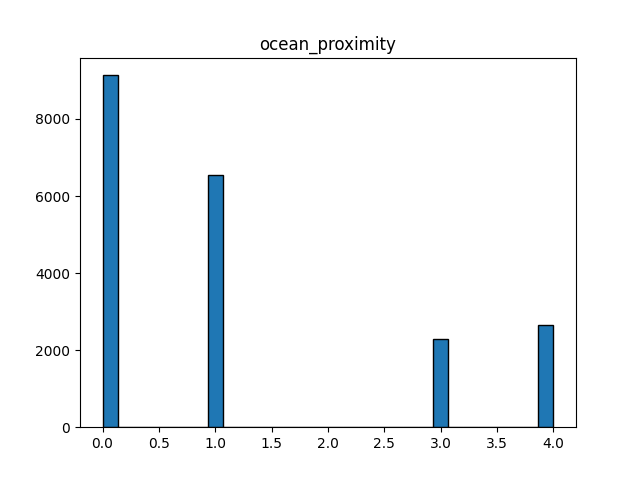
\includegraphics[width=\linewidth]{figs/ocean_proximity_distribution.png}
        \caption{Ocean proximity distribution}
        \label{fig:ocean_proximity_distribution}
    \end{minipage}
\end{figure}

\end{document}
